\documentclass[11pt]{article}\usepackage[]{graphicx}\usepackage[usenames,dvipsnames]{xcolor}
% maxwidth is the original width if it is less than linewidth
% otherwise use linewidth (to make sure the graphics do not exceed the margin)
\makeatletter
\def\maxwidth{ %
  \ifdim\Gin@nat@width>\linewidth
    \linewidth
  \else
    \Gin@nat@width
  \fi
}
\makeatother

\definecolor{fgcolor}{rgb}{0.345, 0.345, 0.345}
\newcommand{\hlnum}[1]{\textcolor[rgb]{0.686,0.059,0.569}{#1}}%
\newcommand{\hlstr}[1]{\textcolor[rgb]{0.192,0.494,0.8}{#1}}%
\newcommand{\hlcom}[1]{\textcolor[rgb]{0.678,0.584,0.686}{\textit{#1}}}%
\newcommand{\hlopt}[1]{\textcolor[rgb]{0,0,0}{#1}}%
\newcommand{\hlstd}[1]{\textcolor[rgb]{0.345,0.345,0.345}{#1}}%
\newcommand{\hlkwa}[1]{\textcolor[rgb]{0.161,0.373,0.58}{\textbf{#1}}}%
\newcommand{\hlkwb}[1]{\textcolor[rgb]{0.69,0.353,0.396}{#1}}%
\newcommand{\hlkwc}[1]{\textcolor[rgb]{0.333,0.667,0.333}{#1}}%
\newcommand{\hlkwd}[1]{\textcolor[rgb]{0.737,0.353,0.396}{\textbf{#1}}}%
\let\hlipl\hlkwb

\usepackage{framed}
\makeatletter
\newenvironment{kframe}{%
 \def\at@end@of@kframe{}%
 \ifinner\ifhmode%
  \def\at@end@of@kframe{\end{minipage}}%
  \begin{minipage}{\columnwidth}%
 \fi\fi%
 \def\FrameCommand##1{\hskip\@totalleftmargin \hskip-\fboxsep
 \colorbox{shadecolor}{##1}\hskip-\fboxsep
     % There is no \\@totalrightmargin, so:
     \hskip-\linewidth \hskip-\@totalleftmargin \hskip\columnwidth}%
 \MakeFramed {\advance\hsize-\width
   \@totalleftmargin\z@ \linewidth\hsize
   \@setminipage}}%
 {\par\unskip\endMakeFramed%
 \at@end@of@kframe}
\makeatother

\definecolor{shadecolor}{rgb}{.97, .97, .97}
\definecolor{messagecolor}{rgb}{0, 0, 0}
\definecolor{warningcolor}{rgb}{1, 0, 1}
\definecolor{errorcolor}{rgb}{1, 0, 0}
\newenvironment{knitrout}{}{} % an empty environment to be redefined in TeX

\usepackage{alltt}
\usepackage[sc]{mathpazo} 
\usepackage{fullpage}
\usepackage{natbib}
\linespread{1.5}
\usepackage[utf8]{inputenc}
\usepackage{lineno}
\usepackage{titlesec}
\titleformat{\section}[block]{\Large\bfseries\filcenter}{\thesection}{1em}{}
\titleformat{\subsection}[block]{\Large\itshape\filcenter}{\thesubsection}{1em}{}
\titleformat{\subsubsection}[block]{\large\itshape}{\thesubsubsection}{1em}{}
\titleformat{\paragraph}[runin]{\itshape}{\theparagraph}{1em}{}[. ]\renewcommand{\refname}{Literature Cited}
% my addnl packages
\usepackage{geometry}
\usepackage{graphicx}
\usepackage[T1]{fontenc}
\usepackage{authblk}
\usepackage{setspace}
\usepackage{amsfonts,amssymb,amsmath,hyperref}
\usepackage{float}
\usepackage{caption}
\usepackage{multirow}
\usepackage{hyperref}
\usepackage{wrapfig}
\usepackage{rotating}
\usepackage[usenames,dvipsnames]{xcolor}
\newcommand{\revise}[1]{{\color{Mahogany}{#1}}}
\usepackage[normalem]{ulem}
\graphicspath{{/Users/jm200/Library/CloudStorage/Dropbox/Miller Lab/github/POAR-Forecasting/Manuscript/Figures/}}
\newcommand{\tom}[2]{{\color{red}{#1}}\footnote{\textit{\color{red}{#2}}}}


\doublespacing



%-------------------------------------------------------------------------
\title{Forecasting range shifts of a dioecious plant species under climate change}

\author[1]{Jacob K. Moutouama}
\author[2]{Aldo Compagnoni}
\author[1]{Tom E.X. Miller}
\affil[1]{Program in Ecology and Evolutionary Biology, Department of BioSciences, Rice University, Houston, TX USA}
\affil[2]{Institute of Biology, Martin Luther University Halle-Wittenberg, Halle, Germany; and German Centre for Integrative Biodiversity Research (iDiv), Leipzig, Germany}
%-------------------------------------------------------------------------
\IfFileExists{upquote.sty}{\usepackage{upquote}}{}
\begin{document}
%\SweaveOpts{concordance=TRUE}
\maketitle
\noindent{} $\ast$ Corresponding author: jmoutouama@gmail.com\\
\noindent{} Submitted to \textit{Ecology letters}\\
\noindent{} Manuscript type: Article\\
\noindent{} Open Research statement: All of our data and code are available during peer review at \url{https://github.com/jmoutouama/POAR-Forecasting}. This manuscript and its contents can be reproduced from this file: \url{https://github.com/jmoutouama/POAR-Forecasting/Manuscript/Forescasting.Rnw}. All data are provided at \url{https://github.com/jmoutouama/POAR-Forecasting/tree/main/data}.
%\SweaveOpts{concordance=TRUE}

\linenumbers
%-------------------------------------------------------------------------
\newpage
\section*{Abstract}
Sex-specific response to rising temperature and drought raises the questions of whether global change could lead to a drastic change in the sex ratio and whether that change in the sex ratio could drive population extinction or population range shift in dioecious species.
Answering these questions requires an understanding of the mechanism by which a change in vital rates under future climate conditions for both male and female, could be translated into a significant change in population dynamics.
We forecast range shift for a dioecious species using matrix models. 


%-------------------------------------------------------------------------
\section*{Keywords}
climate change, demography, forecasting, matrix projection model, mechanistic models, sex ratio, range limits

%--------------------------------------------------------------------
\newpage
\section*{Introduction}
Rising temperatures and extreme drought events associated with global climate change are leading to increased concern about how species will become redistributed across the globe under future climate conditions \citep{bertrand2011changes,gamelon2017interactions,smith2024extreme}.
Dioecious species (most animals and many plants) might be particularly vulnerable to the influence of climate change because they often display skewed sex ratios that are generated or reinforced by sexual niche differentiation (distinct responses of females and males to shared climate drivers) \citep{Tognetti2012}. 
Accounting for such a niche differentiation within a population is a long-standing challenge in accurately predicting which sex will successfully track environmental change and how this will impact population viability and range shifts \citep{jones1999sex,gissi2023exploring}. 
The vast majority of theory and models in population biology, including those used to forecast biodiversity responses to climate change, ignore the complication of sex structure \citep{pottier2021sexual,ellis2017does}.
As a result, accurate forecasts of colonization-extinction dynamics for dioecious species under future climate scenarios are limited. \tom{}{This is a great opening paragraph!} 

\tom{Climate change can influence dioecious populations via shifts in sex ratio.}{This paragraph is really good but notice that the topic sentence (and much that follows) is largely redundant with the first paragraph. I would suggest creating clearer distinction between paragraphs.} 
Females and males may respond differently to climate change, especially in species where there is sexual niche differentiation \citep{gissi2023exploring,gissi2023sex,hultine2016climate}. 
This sex-specific response to climate change may help one sex to succeed in extreme climatic conditions rather than the other sex \citep{zhao2012sex, burli2022environmental} leading to a skewness in the operational sex ratio (relative number of males and females as available mates) \citep{eberhart2017sex}.
For example, experiments in two populations of Atlantic marine copepods (\textit{Acartia tonsa}) revealed that male survival was more sensitive to increasing temperatures than female survival \citep{sasaki2019complex}.
In other species, such as \textit{Pteropus poliocephalus} or \textit {Populus cathayana}, females showed lower survival than males in response to high temperature \citep{welbergen2008climate,zhao2012sex}. 
Sex-specific responses to climate drivers have the potential to influence population viability under global change because skew in the operational sex ratio can limit reproduction through mate scarcity \citep{petry2016sex}.

Species's range limits, when not driven by dispersal limitation, should generally \tom{reflect the limits of the ecological niche}{cite -- there is a relevant paper by Julie Lee-Yaw and Amy Angert, and lots of related literature}. 
For most species, niches and geographic ranges are often limited by climatic factors including temperature and precipitation \citep{sexton2009evolution}. 
Therefore, any substantial changes in the magnitude of these climatic factors in a given location across the range could impact population viability, with implications for range shifts based on which regions become more or less suitable  \citep{davis2001range, pease1989model}. 
Forecasting range shifts for dioecious species is complicated by the potential for each sex to respond differently to climate variation \citep{pottier2021sexual,morrison2016causes}.
Populations in which males are rare under current climatic conditions could experience low reproductive success due to sperm or pollen limitation that may lead to population decline in response to climate change that disproportionately favors females \citep{eberhart2017sex}.
In contrast, climate change could expand male habitat suitability (e.g. upslope movement), which might increases seed set for pollen-limited females and favor range expansion \citep{petry2016sex}.
Although the response of species to climate warming is an urgent and active area of research, few studies have disentangled the interaction between sex and climate drivers to understand their combined effects on population dynamics and range shifts.  

\tom{Our ability to track the impact of climate change on the population dynamics of dioecious plants and the implication of such impact on range shift depends on our ability to build mechanistic models that take into account the spatial and temporal context in which sex specific response to climate change affects population viability \citep{davis2001range,evans2016towards,czachura2020demographic}.}{This is a great topic sentence and an important point, but the paragraph does not really expand upon this point about mechanistic models. The next few sentences do not really say anything new. I think it would be stronger to discuss the value and challenges of mechanistic models for species' range shifts.}
At their range edge where climatic conditions are expected to be less favorable, if dioecious species populations are non-viable in response to climate change, global warming will induce range contraction in dioecious species.
In reverse, if populations at the edge are viable habitats in response to global warming, dioecious species populations could shift their range and relocate to more favorable and thereby favored range expansion. 

In this study, we used a mechanistic approach by combining geographically-distributed field experiments, hierarchical statistical modeling, and two-sex population projection modeling to understand the demographic response of dioecious species to climate change and its implications for future range dynamics.
Our study system is a dioecious plant species (\textit{Poa arachnifera}) distributed along environmental gradients in the south-central US corresponding to variation in temperature across latitude and precipitation across longitude (MAP). \tom{}{I would include a few more sentences of context about the study before jumping to the questions. For example it seems relevant to acknowledge the previous study and highlight that our previous approach used proxy variables, so could not be used to forecast responses to environmental change.}
% A previous study showed that, despite the differentiation of the climatic niche between sexes, the female niche mattered the most in driving the environmental limits of population viability \citep{miller2022two}. 
Here, we asked four questions: 
\begin{enumerate}
	\item What are the sex-specific vital rate responses to variation in temperature and precipitation across the species' range?
	\item How sex-specific vital rates combine to determine the influence of climate variation on population viability ($\lambda$)?
	\item What are the historical and projected changes in climate across the species range?
	\item What are the back-casted and fore-casted dynamics of this species' geographic niche ($\lambda \geq 1$) and how does accountind for sex structure modify these predictions?
\end{enumerate}

%--------------------------------------------------------------------
\section*{Materials and methods}

\subsection*{Study species}
Texas bluegrass (\textit{Poa arachnifera}) is a perennial, summer-dormant cool-season (C3) grass that occurs in Texas, Oklahoma, and southern Kansas, USA \citep{hitchcock1971manual}. 
Texas bluegrass grows between October and May, with onset of dormancy often from June to September \citep{kindiger2004interspecific}.
Flowering occurs in May and the species is pollinated by wind \citep{hitchcock1971manual}.\tom{}{I think you need to say more about the geographic region and its climate. It will be important to motivate the split of growing and dormant seasons based on the natural history. You also need to describe the reproductive biology including dioecy and wind-pollination.}

\subsection*{Common garden experiment}
We set up a common garden experiment throughout and beyond the range of Texas bluegrass to enable study of sex-specific demographic responses to climate and the implications for range shifts \tom{\citep{merow2017climate,schwinning2022common}. }{I am not sure why you cite these studies here. They would be more appropriate for the Intro if you expand the paragraph about mechanistic modeling.}
Details of the experimental design are provided in \cite{miller2022two}; we provide a brief overview here. 

The common experiment was installed at 14 sites across a \tom{precipitation gradient}{While the Am Nat paper focused on precipitation, the actual design spans both temperature and precip, whch is a feature you can exploit for your analysis, and would be worth highlighting as a source of novelty of this paper relative to the previous one. Some reviewers will be skeptical that we are publishing another paper from the same experiment, so the distinction should be made clear.} (FigX). 
At each site, we established 14 blocks. 
For each block we planted three female and three male individuals that were clonally propagated from eight natural source populations of Texas bluegrass. 
The experiment was established in November 2013 and was census annually through 2016, providing both spatial and inter-annual variation in climate. 

In mid-May of each year (2014-2016), we collected individual demographic data including survival (alive or dead), growth (number of tillers), flowering status (reproductive or vegetative), and fertility (number of panicles, conditional on flowering). 
For the analyses that follow, we focus on the 2014-15 and 2015-16 transitions years, since 2013-14 was not a complete (12-month) transition year. 
The data set included \# unique individuals (\# and \# females) and \# plant-year observations. 

\subsection*{Climatic data collection}
We downloaded monthly temperature and precipitation from Chelsa to describe observed climate conditions during our study period \citep{karger2017climatologies}.
These climate data were used as covariates in vital rate regressions, which allowed us to forecast and back-cast demographic responses to climate change based on observations across the common garden experiment. 
%We prefer temperature and precipitation because they capture the most the climate in the study region \colorbox{BurntOrange}{Source}. 
We aligned the climatic years to match demographic transition years \tom{(June 1 -- May 31)}{Updated with new approach.} rather than calendar years.
Based on the natural history of this summer-dormant cool-season species, we divided each transition year into growing and dormant seasons. 
We define June 1 through September 30 as the dormant season and the rest of the transition year (October 1 -- May 31) as the growing season. 
Across years and sites, the experiment included substantial variation in growing and dormant season temperature and precipitation (Figure \ref{fig:site_year_weather}).

To back-cast and forecast changes in climate, we downloaded projection data for three 30-year periods: past (1901-1930), current (1990-2019) and future (2070-2100).
Data for these climatic periods were downloaded from four general circulation models (GCMs) selected from the Coupled Model Intercomparison Project Phase 5 (CMIP5). 
The GCMs are MIROC5, ACCESS1-3, CESM1-BGC, CMCC-CM  and were downloaded from chelsa \citep{sanderson2015representative}.
We evaluated future climate projections from two scenarios of representative concentration pathways (RCPs): RCP4.5, an intermediate-to-pessimistic scenario assuming a radiative forcing to amount to 4.5 $W m^{-2}$ by 2100, and RCP8.5, a pessimistic emission scenario which project a radiative forcing to amount to 8.5 $W m^{-2}$ by 2100 \citep{thomson2011rcp4, schwalm2020rcp8}.

\tom{}{Tom stopped here during the first round of edits. Generall impressions so far: really good! Need more hypotheses regarding sex-specific responses. Also need to say a little more about prev study (including what is known about sex-specific niches), and lean into the natural history at the end of intro and start of methods.}

\subsection*{Sex ratio experiment}
We conducted an experiment at a site near the center of the range to estimate the effect of sex ratio variation on female reproductive success.
Details of the experiment are provided in \cite{compagnoni2017can} and \cite{miller2022two}.
In short, we established 124 experimental populations on plots measuring 0.4 x 0.4m and separated by at least 15m from each other. 
We chose 15m because our pilot data show that more than 90\% of wind pollination occurred within 13m. 
We varied population density (1-48 plants/plot) and sex ratio (0\%-100\% female) across the experimental populations, and we replicated 34 combinations of density and sex ratio. 
We collected the number of panicles from a subset of females in each plot and recorded the number of seeds in each panicle. 
The raw seed count included both fertilized and unfertilized seeds.  
We further assessed reproductive success (seeds fertilized) using greenhouse-based germination and trazolium-based seed viability assays. 

Using these data, seed viability was modeled as a function of local sex ratio with a binomial distribution where the probability of viability ($v$) was given by:
\begin{align}\label{eq:viab_fn}
v = v_{0} * (1 - OSR^{\alpha})
\end{align}
\noindent $OSR$ is the operational sex ratio (proportion of panicles that were female) in the experimental populations.
The properties of this function are supported by our previous work \citep{compagnoni2017can}: seed viability is maximized at $v_{0}$ as $OSR$ approaches zero (strongly male-biased) and goes to zero as $OSR$ approaches $1$ (strongly female-biased).
Parameter $\alpha$ controls how viability declines with increasing female bias.

We used a binomial distribution to model the germination data from greenhouse trials.
Given that germination was conditional on seed viability, the probability of success was given by the product $v*g$, where $v$ is given by Eq. \ref{eq:viab_fn} and $g$ is assumed to be constant.

\subsection*{Sex specific demographic responses to climate}
We used individual-level measurements of survival, growth (number of tillers), flowering, and number of panicles to develop Bayesian mixed effect models describing how each vital rate varies as a function of sex, size, and temperature and precipitation of growing and dormant seasons. 
To allow for non-monotonic climate responses (e.g., intermediate optima), we fit vital rate models with second-degree polynomial functions for the influence of climate variables.
We account for background heterogeneity associated with site, block, and source population of the transplants, which are modeled as statistical random effects.

All the vital rate models used the same linear predictor for the expected value ($\mu$)(Eq. \ref{eq:mu}) that included main effects of size, sex, and four climate variables as well as two-way and three-way interactions that allow for interaction between temperature and precipitation (within season) and sex-specific size-dependence and climate-sensitivity:
\begin{align}\label{eq:mu}
\begin{split}
f(\mu) = \beta_{0} + \beta_{1}size + \beta_{2}sex + \beta_{3}pptgrow + \beta_{4}pptdorm + \beta_{5}tempgrow + \beta_{6}tempdorm \\ 
+ \beta_{7}pptgrow*sex + \beta_{8}pptdorm*sex + \beta_{9}tempgrow*sex + \beta_{10}tempdorm*sex  \\ 
+  \beta_{11}size*sex + \beta_{12}pptgrow*tempgrow + \beta_{13}pptdorm*tempdorm\\
+ \beta_{14}pptgrow*tempgrow*sex + \beta_{15}pptdorm*tempdorm*sex + \beta_{16}pptgrow^2\\
+ \beta_{17}pptdorm^2 + \beta_{18}tempgrow^2 + \beta_{19}tempdorm^2 + \beta_{20}pptgrow^2*sex  \\
+ \beta_{21}pptdorm^2*sex + \beta_{22}tempgrow^2*sex + \beta_{23}tempdorm^2*sex + \phi + \rho + \nu 
\end{split}
\end{align}
\noindent When used as a covariate, $size$ was on a natural logarithm scale ($log(tillers)$). 
We centered and standardized (mean zero, unit variance) all predictors to facilitate model convergence.
$pptgrow$ is the precipitation of the growing season, $tempgrow$ is the temperature of the growing season, $pptdorm$ is the precipitation of the dormant season, $tempdorm$ is the temperature of the dormant season.
The model also includes normally distributed random effects for site to site variation ($\nu \sim N(0,\sigma_{site})$), block-to-block variation ($\phi \sim N(0,\sigma_{block})$), and variation among source populations related to the provenence of the plants used to establish the common garden ($\rho \sim N(0,\sigma_{source})$), 

We applied a different link function ($f(\mu)$) and error distribution depending on the vital rate. 
We modeled survival and flowering data with a Bernoulli distribution (logit link).
We modeled the growth (tiller number) with a zero-truncated Poisson inverse Gaussian distribution and fertility (panicle count) as zero-truncated negative binomial (log link). 
For growth and survival the size covariate was log(tillers) in the previous census. 
For flowering and panicle production the size covariate was log(tillers) in the current census. 
Note that the growth model uses raw tiller count as the discrete response variable, which allows us to populate a transition matrix for expected tiller number conditional on previous tiller number. 
We found that the mean-variance flexibility of the Poisson inverse Gaussian was necessary for capturing patterns of size transition in the data. 

We fit all models in Stan \citep{rstan}, with weakly informative priors for all $\beta$ coefficients ($\mu = 0, \sigma = 100$) and variances ($\gamma [0.001, 0.001]$). 
We ran three chains for 1000 samples for warmup and 4000 for interactions, with a thinning rate of 3. 
We used trace plots to assess model convergence and predictive checks to compare real data against data simulated from the fitted models \citep{piironen2017comparison} (Appendix S1: Figure S1).
\tom{To understand the effect of climate on vital rates, we got the 95 \% credible interval of the posterior distribution.}{Because there are quadratic terms in the model I don't think the coefficients really tell the story of climate effects. It's much more effective to look at your plots of the functions, though it could still be fine to include the coefficient plot in the appendix. One concern: there are 24 coefficients in the model you have written above but only 21 in the Posterior\_mean.pdf coefficient plot.}  

\subsection*{Population growth rate responses to climate}
To understand the effect of climate on population growth rate, we used the fitted vital rates to build a matrix projection model (MPM) structured by size (number of tillers) and sex, with climate variables as covariates to the vital rate functions. 
Following parameter estimation from the common garden experiment, we assume that demographic sensitivity to climate is limited to survival, growth, the probability of flowering, and panicle production of flowering plants.  
Let $F_{x,t}$ and $M_{x,t}$ be the number of female and male plants of size $x$ in year $t$, where $x \in \{1,2,...,U\}$ and $U$ is the maximum number of tillers a plant can reach (here 95th percentile of observed maximum size).
Let $F^{R}_{t}$ and $M^{R}_{t}$ be the new recruits, which we assume do not reproduce in their first year, and let $\mathbf{z}$ be a vector of climate covariates (growing and dormant season temperature and precipitation).
For a pre-breeding census, the expected numbers of recruits in year $t+1$ is given by:
\begin{align}\label{eq:recruits}
F^{R}_{t+1} = \sum_{x=1}^{U} 	[ \, p^{F}(x;\mathbf{z}) \cdot c^{F}(x;\mathbf{z}) \cdot d \cdot v(\mathbf{F_{t}},\mathbf{M_{t}}) \cdot m \cdot \rho 	] \, F_{x,t}
\\
M^{R}_{t+1} = \sum_{x=1}^{U} 	[ \, p^{F}(x;\mathbf{z}) \cdot c^{F}(x;\mathbf{z}) \cdot d \cdot v(\mathbf{F_{t}},\mathbf{M_{t}}) \cdot m \cdot (1-\rho) 	] \, F_{x,t}
\end{align}

\noindent where $p^{F}$ and $c^{F}$ are flowering probability and panicle production for females of size $x$, $d$ is the number of seeds per female panicle, $v$ is the probability that a seed is fertilized, $m$ is the probability that a fertilized seed germinates, and $\rho$ is the primary sex ratio (proportion of recruits that are female), $z$ is the climate. 
Seed fertilization depends on the OSR of panicles (following Eq. \ref{eq:viab_fn}) which was derived from the $U \times 1$ vectors of population structure $\mathbf{F_{t}}$ and $\mathbf{M_{t}}$:
\begin{align}\label{eq:viab_MPM}
v(\mathbf{F_{t}},\mathbf{M_{t}}) = v_{0} * \left[ 1 - \left( \frac{\sum_{x=1}^{U} p^{F}(x;\mathbf{z}) c^{F}(x;\mathbf{z}) F_{x,t}}{\sum_{x=1}^{U} p^{F}(x;\mathbf{z}) c^{F}(x;\mathbf{z}) F_{x,t} + p^{M}(x;\mathbf{z}) c^{M}(x;\mathbf{z}) M_{x,t}} \right) ^{\alpha}\right]
\end{align}

Thus, the dynamics of the size-structured component of the population are given by:
\begin{align}\label{eq:dynamics}
F_{y,t+1} = [ \, \sigma \cdot g^{F}(y,x=1;\mathbf{z}) ] \, F^{R}_{t} + \sum_{x=1}^{U} 	[ \, s^{F}(x;\mathbf{z}) \cdot g^{F}(y,x;\mathbf{z})] \, F_{x,t}
\\
M_{y,t+1} = [ \, \sigma \cdot g^{M}(y,x=1;\mathbf{z}) ] \, M^{R}_{t} + \sum_{x=1}^{U} 	[ \,  s^{M}(x;\mathbf{z}) \cdot g^{M}(y,x;\mathbf{z}) ] \, M_{x,t}
\end{align}

\noindent In Eq. \ref{eq:dynamics}, the first term represents seedlings that survived their first year (survival probability $\sigma$) and enter the size distribution of established plants.
Because we did not measure \textit{P. arachnifera} seedling survival in our common garden experiment, we used the seedling survival probability from our demographic studies of the hermaphroditic congener \textit{Poa autumnalis} in east Texas (\textit{unpublished data}), and we assume this probability was constant across sexes and climatic variables. 
%We did this because we had little information on the early life cycle transitions of greenhouse-raised transplants.
We also assume that surviving seedlings reach size $y$ in year $t+1$ according to $g(y,x=1;\mathbf{z})$, the expected future size of 1-tiller plants from the common garden experiment.
The second term represents survival and size transition of established plants from the previous year, where $s$ and $g$ give the probabilities of surviving at size $x$ and growing from sizes $x$ to $y$, respectively, and superscripts indicate that these functions may be unique to females ($F$) and males ($M$).

\tom{Because the two-sex MPM is nonlinear (vital rates affect and are affected by population structure) we estimated the asymptotic geometric growth rate ($\lambda$) by numerical simulation, and repeated this across a range of climate.}{I think methods for projecting across a range of climate need to be described in greater detail. Also you say here at you analyzed the two-sex IPM through simulation but the female-dominant version can be analyzed through eigenanalysis, and I think you are presenting both, so this should be explained.}

\subsection*{Identifying the mechanisms of population growth rate sensitivity to climate }
\tom{}{I don't think the LTRE analysis is adequately motivated by the Intro. I have not edited much here but we can talk about it.}
To identify the mechanism by which climate affects population growth rate, we decomposed the effect of each climate variable (here Climate) on population growth rate ($\lambda$) into contribution arising from the effect on each stage-specific vital rate \citep{caswell2000matrix}.
At this end we used a life table response experiment (LTRE) with a regression designs. 
The LTRE approximates the change in $\lambda$ with climate  as the product of the sensitivity of $\lambda$ to the parameters times the sensitivity of the parameters to climate, summed over all parameters \citep{caswell1989analysis}:
\begin{align}\label{eq:ltre}
\frac{\partial \lambda}{\partial Climate} \approx \sum_{i} \frac{\partial \lambda}{\partial \theta^{F}_{i}} \frac{\partial \theta^{F}_{i}}{\partial Climate} + \frac{\partial \lambda}{\partial \theta^{M}_{i}} \frac{\partial \theta^{M}_{i}}{\partial Climate}
\end{align}

\noindent where, $\theta^{F}_{i}$ and $\theta^{M}_{i}$ represent sex-specific parameters: the regression coefficients for the intercepts and slopes of size-dependent vital rate functions. 
Because LTRE contributions are additive, we summed across vital rates to compare the total contributions of female and male parameters. 

\subsection*{Implication on range shifts}
\tom{}{I think this section should be expanded. In general, you did a great job of presenting the model but you have not effectively communicated how you are using the model to answer your questions.}
To understand the implication of our study on range, we extrapolate population growth using past, current and future climatic data  across the range to map species distributions. 
% Because some population growth rate predictions were unrealistic, we limited our population growth rate values to 30\% more or less than the observed maximum and minimum values.  
Averaging projection of population growth rates was used to reduce uncertainty across climate projections (general circulation models). 

All the analysis were performed in R 4.3.1 \citep{RCoreteam}

\section*{Results}
\tom{}{Since the vital rate results will be updated with the new seasonal covariates I will wait to edit an updated version.}
\subsection*{Sex specific demographic response to climate change}
Most vital rates were strongly climate dependent, but the magnitude of their response differed between sexes suggesting a sex-specific demographic response to climate. 
Survival and growth were strongly more dependent on climate than flowering and panicles Fig.\ref{fig:vital_rates}.
There was a female survival and flowering advantage across all climatic seasons (Figs. 3A-3D, 3I-3K). 
On the contrary, there was a male panicle advantage across all climatic variables (Fig3X-Y). 
Counter-intuitively, there was no sex growth advantage in all season climatic variables (Fig 3E-3H). 

Precipitation of the growing season decreased seasonal survival, whereas temperature of the growing season, precipitation of the dormant season, and temperature of the dormant season increased seasonal survival.
Unlike the probability of survival, the probability of flowering increased with precipitation of the growing season and decreased with precipitation of the growing season and increased with temperature of the growing season, precipitation of the dormant season, and temperature of the dormant season.
This trade-off between survival and flowering provides an insight into the persistence of the species. 
In addition, the number of panicles decreased with precipitation for the growing season and the temperature of the dormant season and increased with the temperature of the growing season and precipitation.
Finally, the precipitation and temperature of the growing season decreased seasonal growth, whereas the precipitation and temperature of the dormant season increased seasonal growth. 

\begin{figure}%[h!]
  \begin{center}
    \includegraphics[width=0.95\linewidth]{Figures/vital_rates.pdf}
  \caption{Sex specific demographic response to climate across species range: A--D, inter-annual probability of survival; E--H, inter-annual growth (change in number of tillers); I--L, probability of flowering; M--P, number of panicles produced given flowering. 
  Points show means by site for females (orange) and males (green). 
  Point size is proportional to the sample size of the mean.
  Lines show fitted statistical models for females (orange) and males (green) based on posterior mean parameter values.
  Lower panels below each data panel show the posterior distribution of the difference between females and males as a function of climate (positive and negative values indicate female and male advantage, respectively); dashed horizontal line shows zero difference.}
  \label{fig:vital_rates}
  \end{center}
\end{figure}

\subsection*{Population growth rate response to climate change}

Consistent with the effect of climate on individual vital rate, we also found an effect of seasonal climate on population growth rate. Precipitation and temperature of the growing season decreased the population growth rate, whereas precipitation and temperature of the dormant season increased the population growth rate. Across all sites, the population growth rate was higher than one, suggesting an increase of population over time.

\begin{figure}%[h!]
  \begin{center}
    \includegraphics[width=0.95\linewidth]{Figures/all_lambda.pdf}
  \caption{XXX}
  \label{fig:vital_rates}
  \end{center}
\end{figure}


%--------------------------------------------------------------------
\newpage
\section*{Appendix S1: Correspondence }
\renewcommand{\thefigure}{A\arabic{figure}}\setcounter{figure}{0}
\renewcommand{\thetable}{A\arabic{table}}\setcounter{table}{0}
\renewcommand{\theequation}{A\arabic{equation}}\setcounter{equation}{0}
	\begin{figure}[H]
		\centering
		\includegraphics[width = \linewidth]{Figures/Varianceexplained.pdf}
		\caption{\textbf{Relation between precipitation and temperature for each season (growing and dormant).} $R^2$ indicates the value of proportion of explained variance between the temperature and precipitation}
	\end{figure}
	
  \begin{figure}[H]
		\centering
		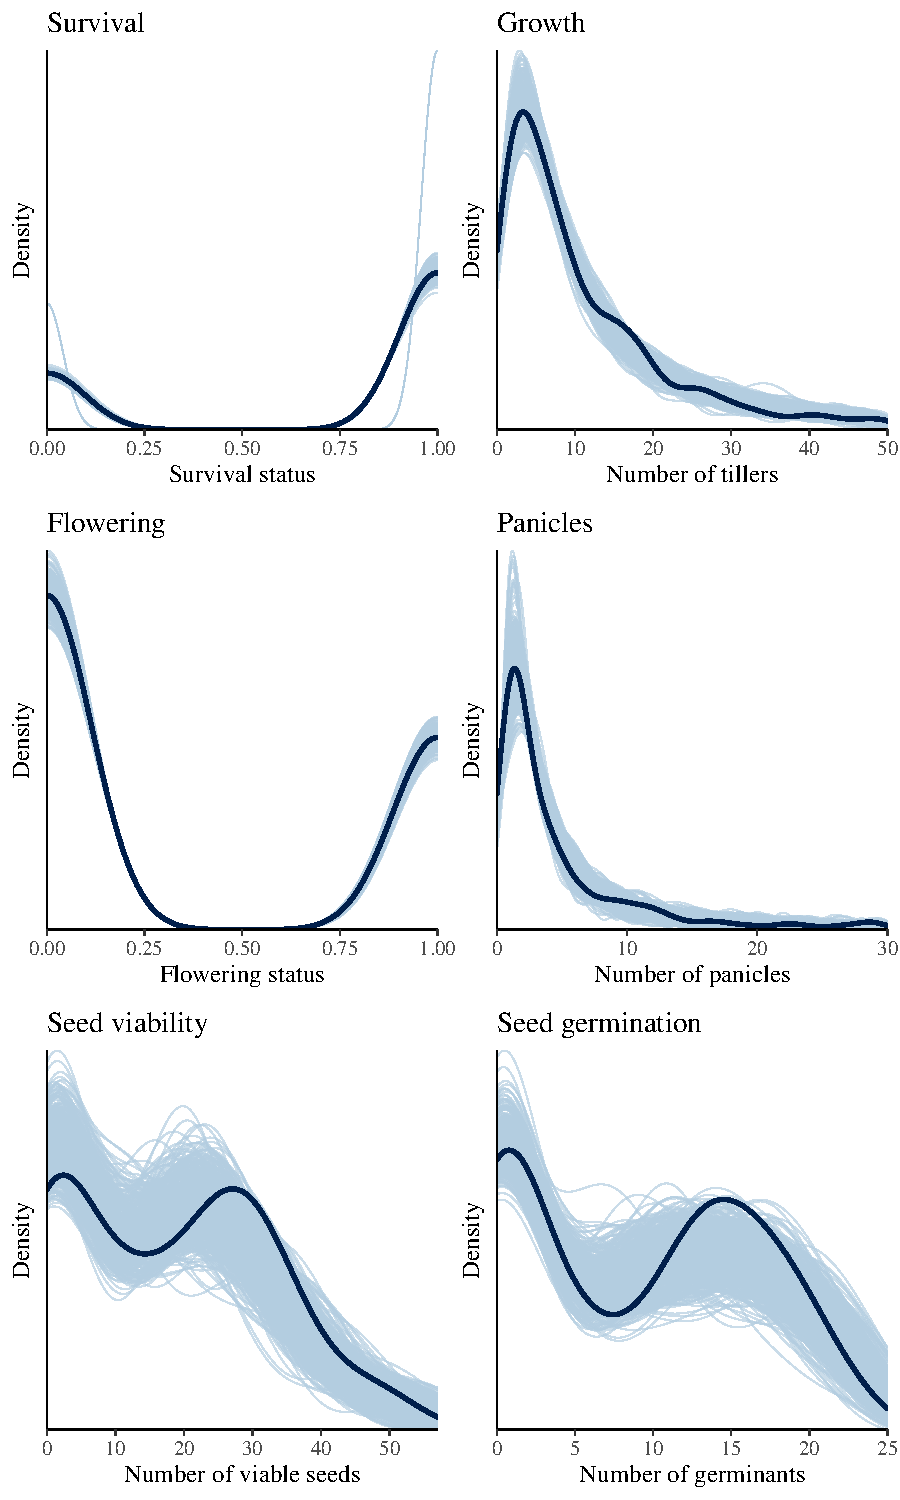
\includegraphics[scale = 0.5]{Figures/PPCtmax_tmin.pdf}
		\caption{\textbf{Consistency between real data and simulated values suggests that the fitted model accurately describes the data}. Graph shows density curves for the observed data (light blue ) along with the simulated values (dark blue). The first column shows the linear models and the second column shows the 2 degree polynomial models.}
	\end{figure}
	
	
	 \begin{figure}%[h!]
		\centering
		\includegraphics[scale = 4.5]{Figures/Posterior_mean.pdf}
		\caption{\textbf{Posterior mean for each vital rate}. }
	\end{figure}
	
\begin{figure}%[h!]
	\begin{center}
		\includegraphics[width=0.95\linewidth]{Figures/site_year_weather.pdf}
		\caption{XXX}
		\label{fig:site_year_weather}
	\end{center}
\end{figure}

\bibliographystyle{ecology}
\bibliography{Forecasting}
\end{document}
